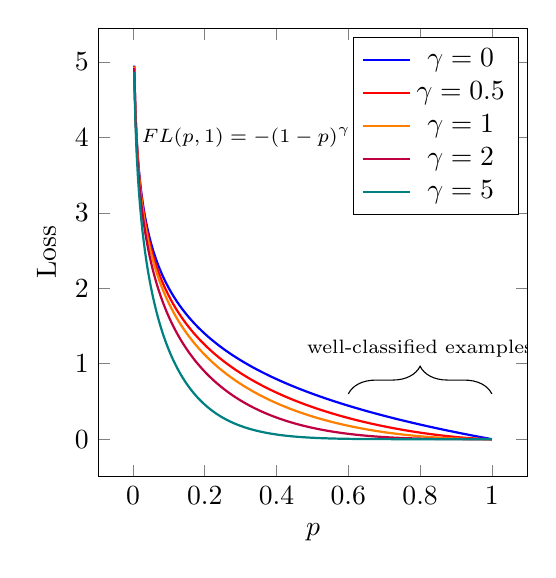
\begin{tikzpicture}
	\begin{axis}[
		xlabel=$p$,
		ylabel=Loss,
		width=0.58\textwidth,
        height=\axisdefaultheight
	]
	
	\addplot[samples=300, domain=0:1, thick, blue]   {2 * -(1-x)^0   * log10(x)};
	\addlegendentry{$\gamma = 0$}
	\addplot[samples=300, domain=0:1, thick, red]    {2 * -(1-x)^0.5 * log10(x)};
	\addlegendentry{$\gamma = 0.5$}
	\addplot[samples=300, domain=0:1, thick, orange] {2 * -(1-x)^1   * log10(x)};
	\addlegendentry{$\gamma = 1$}
	\addplot[samples=300, domain=0:1, thick, purple] {2 * -(1-x)^2   * log10(x)};
	\addlegendentry{$\gamma = 2$}
	\addplot[samples=300, domain=0:1, thick, teal]   {2 * -(1-x)^5   * log10(x)};
	\addlegendentry{$\gamma = 5$}
	
	\node[] at (0.4, 4) {\scriptsize{$\text{FL}(p, 1) = -(1 - p)^{\gamma} \log (p)$}};
	\draw [decorate,decoration={brace,amplitude=10pt}]
	(0.6, 0.6) -- (1, 0.6) node[midway]{};
	\node[] at (0.8, 1.2) {\scriptsize{well-classified examples}};
	\end{axis}
\end{tikzpicture}